\documentclass[a4paper,11pt,notitlepage,hidelinks]{article}

\usepackage{ucs}
\usepackage[utf8x]{inputenc}
\usepackage{amsmath}
\usepackage{amsfonts}
\usepackage{amssymb}
\usepackage{amsthm}
\usepackage{caption}
\usepackage{subfigure}
\usepackage{wrapfig}
\usepackage{fullpage}
\usepackage[usenames]{xcolor}
\usepackage[english]{babel}
\usepackage[T1]{fontenc}
\usepackage{placeins}
\usepackage[pdftex]{graphicx}
\usepackage[pdftex]{hyperref}
\usepackage{tikz}
\usepackage{multicol}
\usepackage[noend,linesnumbered,noresetcount]{algorithm2e}

\usetikzlibrary{calc,decorations.markings,arrows}

\author{Jan Kończak}
\title{JPaxos results}
\date{04.10.2013}

\begin{document}

% Text width: \the\textwidth

\paragraph{Purpose} tests made to see how well the benchamrk has been enhanced \& fixed since september 2013.

\paragraph{Code base} commit 6b0907559c97715660ebbe9cd13e74906bc8a753

\section{Request size versus performance}

\subsection{NIO}
\label{nio}

To get the point when CPU saturates, {1k, 3k, 6k} clients were forced to send requests of sizes from 16 bytes to 512 bytes.
Results, both in rps and bps, are presented below:

\noindent\ignorespaces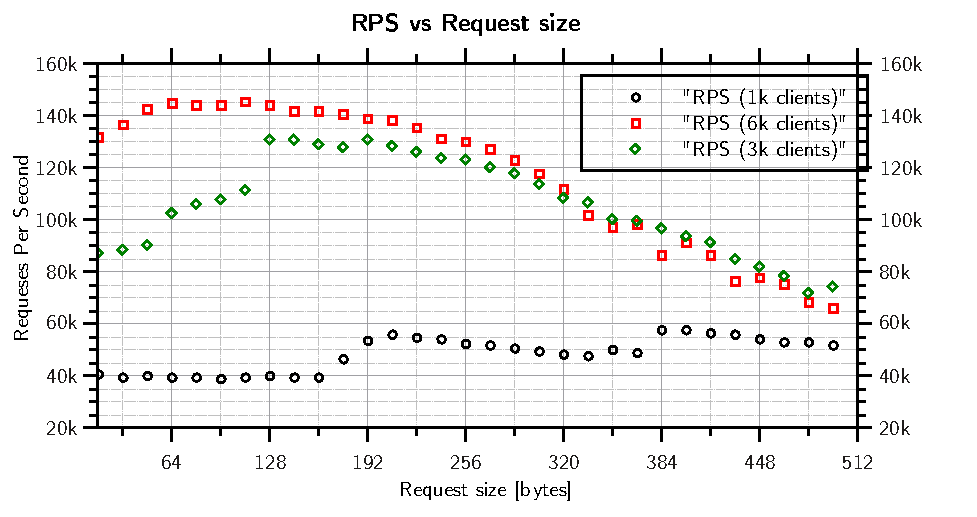
\includegraphics{varsize_rps.pdf}

\noindent\ignorespaces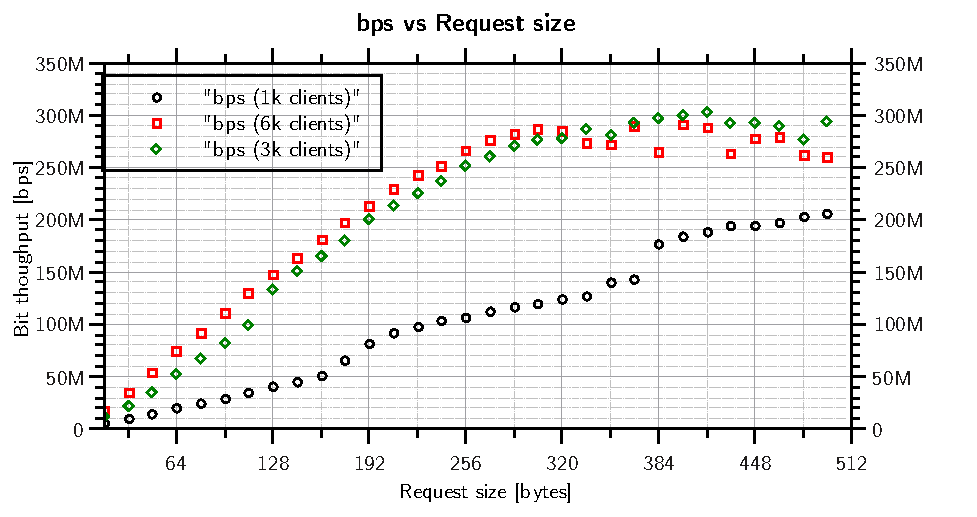
\includegraphics{varsize_bps.pdf}

CPU saturation point has moved from 900b to 320b (i.e., smaller requests saturate network).
1k clients are not able to saturate system even with 512b requests. With 3k and 6k clients, from 192b to 320b the CPU is saturated. Less -- possiblly not enough requests;  more -- network is the limit.

\section{Client count versus performance}

The performance between 3k and 6k clients varied more than expected in previous benchamrk. To see how many clients must send requests to fully saturate JPaxos, te performance with variable client count (3k..12k) for {16, 64, 128, 256} byte requests has been measured. Results below:

\noindent\ignorespaces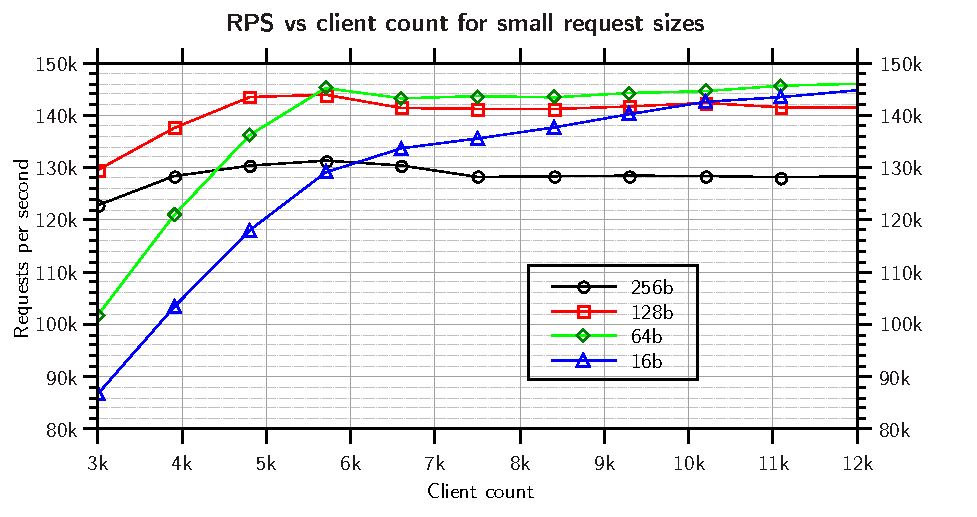
\includegraphics{cliCount_rps.pdf}

6k clients saturate JPaxos sending \textbf{128b} and \textbf{256b} requests -- increasing client count does not improve performance anymore.
With \textbf{64b} there is also a peek at 6k clients; with more clients the throughput first slightly drops, then slightly increases, reaching similar level with 12k clients. The differences in throughput from 6k to 12k clients are however minor.
For \textbf{16b} requests the number of clients needed to saturate JPaxos exceeds the setup -- highest throughput is reached with  the highest client number tested.

\section{TCP vs NIO}

Tests from Section \ref{nio} have been repeated with TCP to see, how faster NIO is. It turned out that NIO is not faster at all:

\noindent\ignorespaces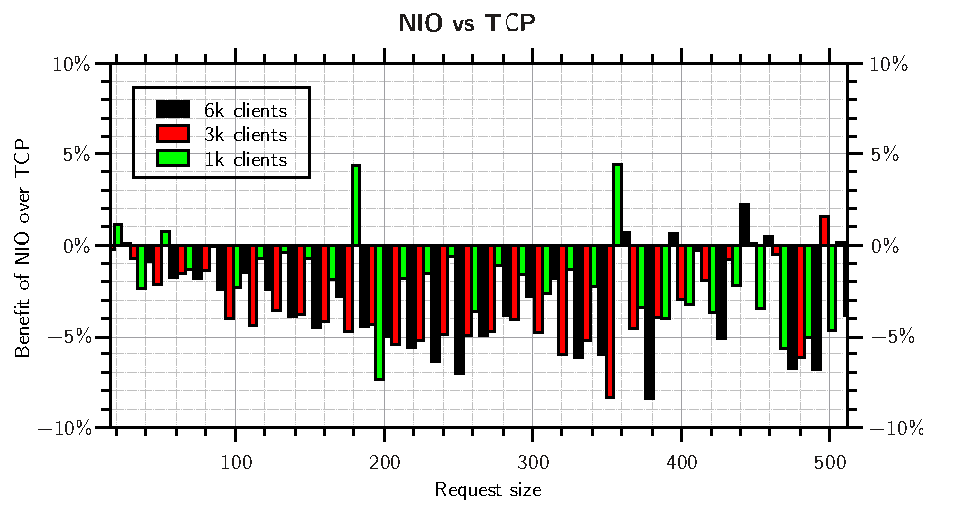
\includegraphics{nio_tcp.pdf}


\end{document}
